\documentclass[]{article}
\usepackage[top=2cm,bottom=2cm,left=2.2cm,right=2.2cm]{geometry}
\usepackage{tikz}
\usepackage{subcaption}
\usepackage{xcolor}
\usepackage[hidelinks]{hyperref}


% Custom TikZ commands
\newcommand{\white}[3] {
  \foreach \x in {0, ..., #3} {
    \draw[fill=white] ({.5+#1},{\x*.1+.5+#2}) circle (0.42) node {#3};
  }
}
\newcommand{\black}[3] {
  \foreach \x in {0, ..., #3} {
    \draw[fill=white!70!black] ({.5+#1},{\x*.1+.5+#2}) circle (0.42) node {#3};
  }
}
\newcommand{\colorSquare}[3] {
  \draw[fill=#1] ({#2},{#3}) rectangle ({#2+1},{#3+1});
}

% for easy game-renaming
\newcommand{\gameName}{Expendibots}


\renewcommand{\abstractname}{}

\title{
{\small\sc
    The University of Melbourne\\
    School of Computing and Information Systems\\
    COMP30024 Artificial Intelligence\\[1.5ex]
}
{\LARGE 
    Project Part A:\\[1ex]
}
{\Huge\bf
    Searching
}
}
\author{}
\date{\normalsize Last updated March 3, 2020}

\begin{document}
\maketitle

\section*{Overview}

In this first part of the project, we will play a single-player variant
of the game of \emph{\gameName}. Before you read this specification,
please make sure you have carefully read the entire `Rules for the Game
of \emph{\gameName}' document.

The aims for Project Part A are for you and your project partner to (1)
refresh and extend your Python programming skills, (2) explore some of
the new algorithms we have met in lectures so far, and (3) become more
familiar with some core mechanics of \emph{\gameName}. This is also a
chance for you to invest some time developing fundamental Python tools
for working with the game: some of the functions and classes you create
now may be helpful later (when you are building your game-playing
program for Project Part B).

\subsection*{Single-player \emph{\gameName}}

The single-player variant of \emph{\gameName} we will analyse works as follows.
You will always play as White, and you will be the only player that acts.
The Black player is static and does not take any turns. As the White player,
you will start with at most 3 tokens in some configuration. You will 
repeatedly take turns until all of the Black tokens have been eliminated, at
which point you win. If on your last turn you eliminate all enemy tokens but
lose your last token, you still win.

\subsection*{The tasks}

Firstly, your team will design and implement a program that `plays' a
game of single-player \emph{\gameName} --- given a board configuration, your
program will find a sequence of actions for the White player to take to win
(to eliminate all enemy tokens). Your program's performance will be judged based
upon its ability to find winning sequences of actions and handle cases involving
multiple tokens (See the Assessment section for details). There is \emph{no} 
requirement that your sequences be optimal.

Secondly, your team will write a brief report discussing and analysing
the strategy your program uses to solve this search problem. These tasks
are described in detail in the following sections.

\section*{The program}

You must create a program to play this game in the form of a Python 3.6
module called \texttt{search}
(for example, a folder named \texttt{search} containing a Python file
called \texttt{\_\_main\_\_.py} as the program entry-point\footnotemark\ 
would be sufficient
--- see the provided skeleton code for a starting point).

\footnotetext{
To run such a Python `module' from the command-line,
begin outside the \texttt{search} folder and use the following command:
`\texttt{python~-m~search}' (followed by command-line arguments).
If \texttt{python} is your Python 3.6 interpreter, it will execute the
code inside \texttt{search/\_\_main\_\_.py}.
}

When executed, your program must read a JSON-formatted board
configuration from a file, calculate a winning sequence of actions, and
print out this sequence of actions. The input and output format are
specified below, along with the coordinate system we will use for both
input and output.

\subsection*{Coordinate system}

The coordinate system in use is a two element pair $(x, y)$ representing the
$x$ (horizontal) and $y$ (vertical) position on the board. This is shown in 
Figure \ref{fig:coordinates}. Note that the coordinates are zero-indexed.

\begin{figure}[ht!]
\centering
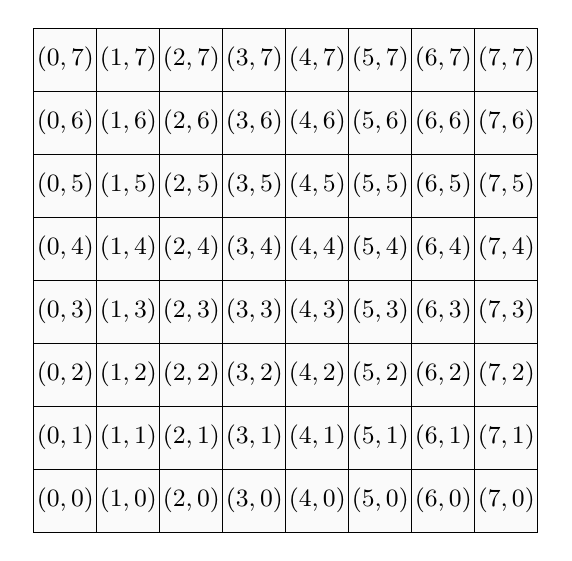
\begin{tikzpicture}[scale=0.8]
\draw[fill=black!2!white] (0, 0) rectangle (8, 8);
\draw[step=1] (0, 0) grid (8, 8);
\foreach \y in {0, ..., 7} {
	\foreach \x in {0, ..., 7} {
		\node[] at ({.5+\x}, {.5+\y}) {\small $(\x, \y)$};
	}
}
\end{tikzpicture}
\caption{Coordinate system for \emph{\gameName}.}
\label{fig:coordinates}
\end{figure}

\subsection*{Input format}
Your program must read a board configuration from a JSON-formatted file.
The name of the file will be given to your program as its first (and
only) command-line argument. The JSON file will contain a single
dictionary (JSON object) with the following 2 entries (name/value
pairs):\footnotemark

\footnotetext{We recommended using Python's Standard Library module
`\texttt{json}' for loading JSON-formatted input data. In this
setting, an appropriate call would be
`\texttt{with open{(}sys.argv{[}1{]}{)} as file: data = json.load(file)}'
(creating \texttt{data}, a dictionary with the input).}


\begin{itemize}
\item
  An entry with key \texttt{"white"} specifying the starting position
  of your player's token(s). The value will be a list (JSON array) of
  \emph{stacks}, with each stack represented in the form \texttt{{[}$n$,$x$,$y${]}}.
  This represents a stack of $n$ tokens at the coordinates $(x, y)$ (as described in
  Figure \ref{fig:coordinates}). For example, the entry \texttt{"white":{[}{[}2,7,0{]}{]}}
  indicates a single stack of two White tokens at $(7, 0)$ (which is the bottom 
  right corner of the board).
\item
  An entry with key \texttt{"black"} specifying the position of your opponent's token(s)
  in the same format.
\end{itemize}

\begin{figure}[ht!]
\centering
\begin{subfigure}[b]{.45\textwidth}
\centering
\begin{verbatim}
{
    "white": [[1,5,3],[1,3,4]],
    "black": [[2,4,6],[1,3,1],[1,5,1]]
}
\end{verbatim}
\vspace{8ex} % Hacky!
\caption{A complete example input file.}
\end{subfigure}
\begin{subfigure}{.08\textwidth}
\phantom{SP}
\end{subfigure}
\begin{subfigure}[b]{.45\textwidth}
\centering
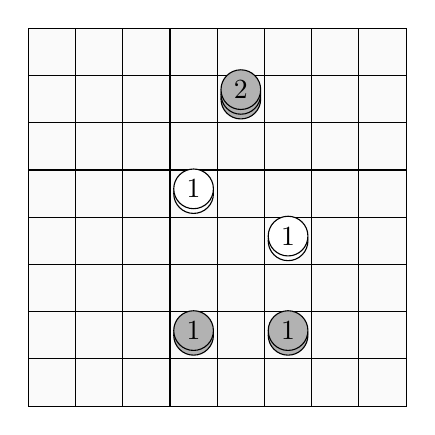
\begin{tikzpicture}[scale=0.6]
	\draw[fill=black!2!white] (0, 0) rectangle (8, 8);
	\draw[step=1] (0, 0) grid (8, 8);
	\white{5}{3}{1};
	\white{3}{4}{1};
	\black{4}{6}{2};
	\black{3}{1}{1};
	\black{5}{1}{1};
\end{tikzpicture}
\caption{The corresponding board configuration.}
\end{subfigure}
\end{figure}

Your program may assume that its input will match this format
specification exactly, and that all stack coordinates represent real
and otherwise unoccupied squares on the board (that is, there will be no
invalid or duplicated coordinates and no improperly formatted JSON in
the input files we provide to your program).

Furthermore, your program may assume that at least one winning sequence
of actions exists for the board configuration described in its input
(that is, your program will not be tested on configurations with no
solution).

\subsection*{Output format}

Your program must print out a winning sequence of actions. Each action
must be allowed according to the rules of the game when played in the
order of output. The actions must be printed to \emph{standard output},
one per line, in the following format:

\begin{itemize}
\item
  To output a move action, print a line in the format
  `\texttt{MOVE\ $n$ from\ ($x_a$,\ $y_a$)\ to\ ($x_b$,\ $y_b$).}'
  where $n$ is the number of tokens in the stack to move, $(x_a, y_a)$
  are the coordinates of the moving tokens before
  the move, and $(x_b, y_b)$ are the coordinates after the move.
  Note: If you want to output the action of moving a whole stack,
  $n$ would just be equal to the number of tokens in the stack.
\item
  To output a boom action, print a line in the format
  `\texttt{BOOM\ at\ ($x$,\ $y$).}'
  where $(x, y)$ are the coordinates of the stack initiating the explosion.
\end{itemize}

Your program \emph{should not print any other lines to standard output}.
If you must print additional output, consider printing to \emph{standard
error} instead. Alternatively, we will ignore lines in standard output
beginning with the character `\texttt{\#}', so you may use this
character to begin any lines of output that are not part of your action
sequence.

\begin{figure}[ht!]
\centering
\begin{subfigure}[b]{.5\textwidth}
\centering
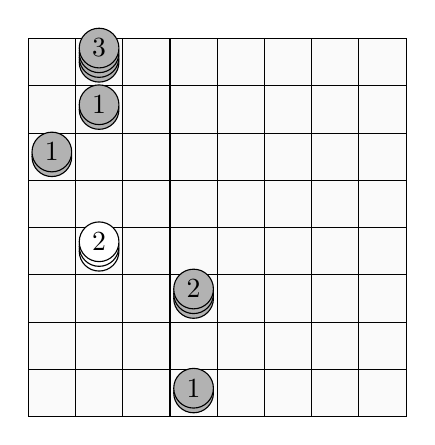
\begin{tikzpicture}[scale=0.6]
	\draw[fill=black!2!white] (0, 0) rectangle (8, 8);
	\draw[step=1] (0, 0) grid (8, 8);
	\white{1}{3}{2};
	\black{3}{0}{1};
	\black{3}{2}{2};
	\black{0}{5}{1};
	\black{1}{6}{1};
	\black{1}{7}{3};
\end{tikzpicture}
\caption{An example board configuration.}
\end{subfigure}
\begin{subfigure}{.08\textwidth}
\phantom{SP}
\end{subfigure}
\begin{subfigure}[b]{.4\textwidth}
\centering
\begin{verbatim}
MOVE 1 from (1, 3) to (1, 1).
MOVE 1 from (1, 1) to (2, 1).
BOOM at (2, 1).
MOVE 1 from (1, 3) to (1, 4).
BOOM at (1, 4).
# lines beginning with # are ignored
# don't forget the full stops!
\end{verbatim}
\vspace{5ex} % Hacky!
\caption{One possible solution output.}
\end{subfigure}
\end{figure}


\section*{The report}

Finally, you must briefly discuss your approach to solving this problem
in a separate file called \texttt{report.pdf} (to be submitted alongside
your program). Your discussion should be structured around the following
3 questions:

\begin{itemize}
\item
  How have you formulated the game as a search problem? (You could
  discuss how you view the problem in terms of states, actions, goal
  tests, and path costs, for example.)
\item
  What search algorithm does your program use to solve this problem, and
  why did you choose this algorithm? (You could comment on the
  algorithm's efficiency, completeness, and optimality. You could
  explain any heuristics you may have developed to inform your search,
  including commenting on their admissibility.)
\item
  What features of the problem and your program's input impact your
  program's time and space requirements? (You might discuss the
  branching factor and depth of your search tree, and explain any other
  features of the input which affect the time and space complexity of
  your algorithm.)
\end{itemize}

Your report can be written using any means but must be submitted as a
PDF document.
Your report should be between 0.5 and 2 pages in length, and must not
be longer than 2 pages.



\newpage

\section*{Assessment}

Your team's Project Part A submission will be assessed out of 8~marks,
and contribute 8\% to your final score for the subject.
Of these 8~marks:

\begin{itemize}
\item
  \textbf{5 marks} will be for the correctness of your program, based on
  running your program through a collection of automated test cases of
  increasing complexity. The test cases will range in difficulty as
  described below, with 1 mark earned by passing the test cases at each
  `level' of difficulty.\footnotemark

  \begin{enumerate}
  \def\labelenumi{\arabic{enumi}.}
  \item
    The player controls 1 White token, and there is 1 Black token.
  \item
    The player controls 1 White token, and there are 2--12 Black tokens.
  \item
    The player controls 2 or 3 White tokens (initially at separate
    squares and with no need to form larger stacks to find a solution),
    and there are 2--12 Black tokens.
  \item
    The player controls 2 or 3 White tokens (possibly in stacks of
    multiple tokens, or with a need to form such stacks),
    and there are 2--12 Black tokens.
  \end{enumerate}

  The 5\textsuperscript{th} mark is earned by correctly adhering to the
  input and output format requirements.
\item
  \textbf{3 marks} will be for the clarity and accuracy of the discussion
  in your \texttt{report.pdf} file, with 1 mark allocated to each of the
  three questions listed above.
  A mark will be deducted if the report is longer than 2~pages or not a
  PDF document.
\end{itemize}

\footnotetext{It may help to break this task down into stages.
For example, begin by implementing a program that can pass tests of
`difficulty level 1' described above, then move on to the higher levels.
Furthermore, even if you don't have a program that works correctly by
the time of the deadline, you should submit anyway.
You may be awarded some marks for making a reasonable attempt.}

\paragraph{Additional notes:}
All tests will be conducted on the \textbf{Melbourne School of
Engineering's student unix machines} (for example, \texttt{dimefox}).
There, your program will be given \textbf{up to 30 seconds} of
computation time per test case. Programs that do not run in this
environment or compute a solution within this time limit will be
considered incorrect. Therefore, we strongly recommended that you test
your program in this environment\footnotemark before submission.
If your team has trouble accessing the student unix machines, please
seek help \emph{well before} submission.

\footnotetext{Note that Python 3.6 is not available on \texttt{dimefox}
by default. However, it can be used after running the command
`\texttt{enable-python3}' (once per login).}

Your program will be run with \textbf{Python 3.6}. For this part of
the project, your program should \textbf{not require any tools from
outside the Python Standard Library}. As one exception to the above,
you may optionally make use of the library of algorithms provided by
the AIMA textbook website (provided you make appropriate
acknowledgements that you have used this library). This library will
be made available to your program in the testing environment if
required.

\subsection*{Academic integrity}

Your submission should be \textbf{entirely the work of your team.}
We automatically check all submissions for originality.
\textbf{Submitting work that is not entirely your own is against the
university's academic integrity policy, and may lead to formal
disciplinary action.}
For example, please note the following:
\begin{enumerate}
\itemsep0ex
\item
You are encouraged to discuss ideas with your fellow students, but
\textbf{it is not acceptable to share code between teams, nor to use
code written by anyone else}.
Do not show your code to another team or ask to see another team's code.
\item
You are encouraged to use code-sharing/collaboration services, such as
GitHub, \emph{within} your team.
However, \textbf{you must ensure that your code is never visible to
students outside your team}.
Set your online repository to `private' mode, so that only your team
members can access it.
\item
You are encouraged to study additional resources to improve your Python
skills.
However, \textbf{any code adapted from an external source must be clearly
acknowledged}.
If you use code from a website, you should include a link to the source
alongside the code.
\end{enumerate}
Please refer to the `Academic Integrity' section of the LMS and to the
university's academic integrity website
(\href{https://academicintegrity.unimelb.edu.au}{\texttt{academicintegrity.unimelb.edu.au}}),
or ask the teaching team,
if you need further clarification.

\section*{Submission}

One submission is required from each team. That is, one team member is
responsible for submitting all of the necessary files that make up your
team's solution.

You must submit a single compressed archive file (e.g.~a \texttt{.zip}
or \texttt{.tar.gz} file) containing all files making up your solution
via the `Project Part A Submission' item in the `Assessments' section of
the LMS. This compressed file should contain all Python files required
to run your program, along with your report.

\begin{center}
\textbf{The submission deadline for Project Part A is 11:00PM on Tuesday
the 7th of April.}
\end{center}

Late submissions are allowed. A late submission will incur a penalty of
two marks per day (or part thereof) late. You may submit
multiple times. We will mark the latest submission made by a member of
your team, unless we are advised otherwise.

\subsection*{Extensions}

If you require an extension, please email \texttt{comp30024-team@unimelb.edu.au}
using the subject `COMP30024 Extension Request' at the earliest possible
opportunity. We will then assess whether an extension is appropriate. Requests
for extensions on medical grounds received after the deadline may be declined.

\end{document}
